\chapter{Theoretical Background \label{chap:2_TheoreticalBackground}}

    %%%%%%%%%%%%%%%%%%
    % Grammarly: 100/100
    %%%%%%%%%%%%%%%%%%
    In this chapter, we present the background of the main concepts regarding our study. The focus is to present the components of an \acl{USV}, and present the international regulations for navigation of vessels on water (\acs{COLREGS}).

\section{GNC System}
    
    %%%%%%%%%%%%%%%%%%
    % Grammarly: 99/100
    %%%%%%%%%%%%%%%%%%
    The \acs{GNC} system is an essential component for most \acp{USV}, being responsible for managing partially or entirely the \ac{USV}. \acs{GNC} stands for Guidance, Navigation, and Control. In this section, we describe the responsibilities of each one of the \ac{GNC} modules as well as the interaction between them. The Figure \ref{fig:Liu2016Unmanned_GNCSystem} presented by Liu~\cite{Liu2016Unmanned} summarize \acs{GNC} modules; their responsibilities and interactions.
    
    \begin{figure}[H]
        \centering
        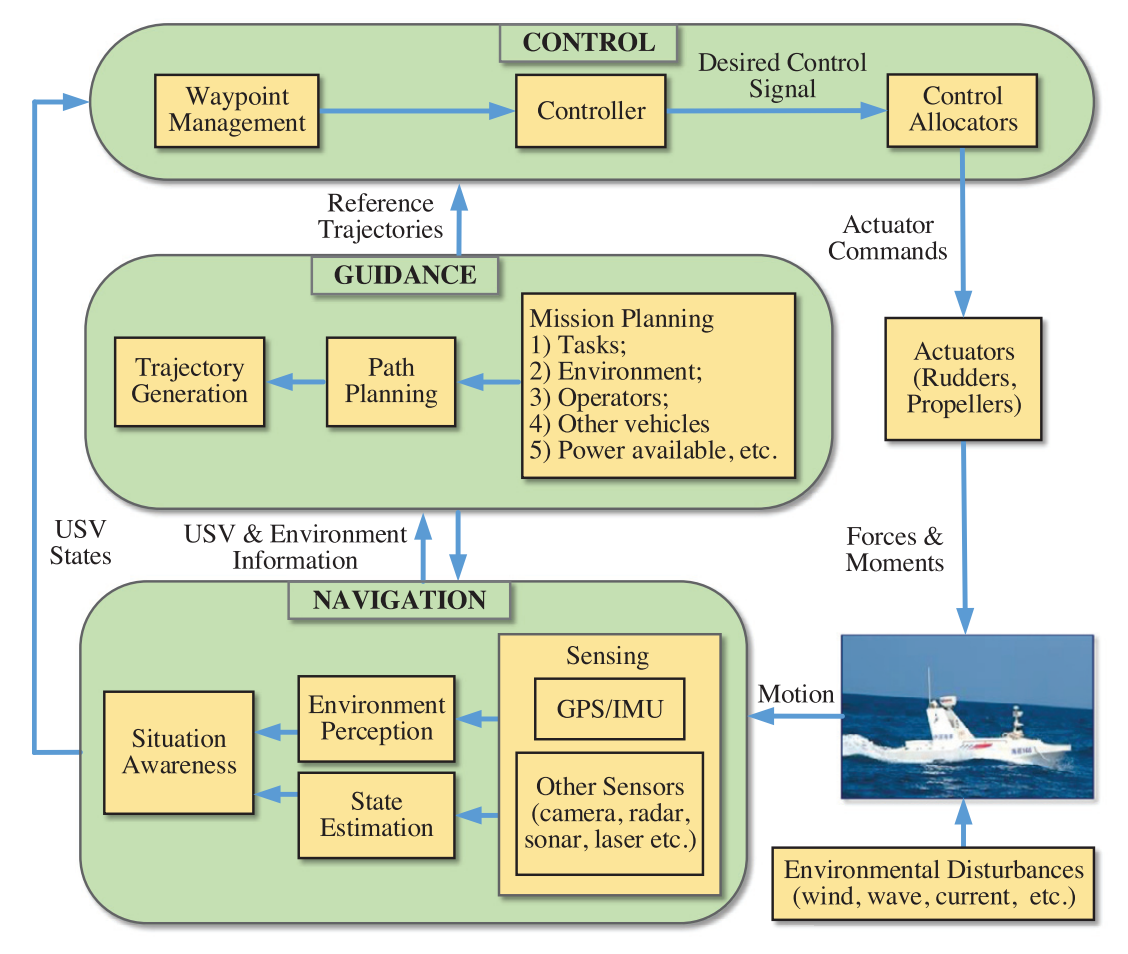
\includegraphics[scale=0.85]{figs/Chap2/Liu2016Unmanned_GNCSystem.png}
        \caption{\ac{GNC} System Modules~\cite{Liu2016Unmanned}}
        \label{fig:Liu2016Unmanned_GNCSystem}
    \end{figure}
    
    %%%%%%%%%%%%%%%%%%
    % Grammarly: 100/100
    %%%%%%%%%%%%%%%%%%
    In short, the guidance system is responsible for the determination of the \ac{USV}'s trajectory to achieve a goal location. For trajectory generation\todo{"For trajectory generation" está certo e é equivalente a "To generate the trajectory"?}, the guidance system uses the information provided by the navigation system regarding the environment (\eg~obstacles around and general disturbances such as wind and current) and related to the \ac{USV}'s state (\eg~current location). After generating the trajectory, the guidance system makes the route available to the control system. The control system generates actuation commands to change the \ac{USV}'s state and effectively move the \ac{USV}. We present detailed explanations about the \ac{GNC} modules in the following sections.
    
    \subsection{Guidance System}
    
    %%%%%%%%%%%%%%%%%%
    % Grammarly: 100/100
    %%%%%%%%%%%%%%%%%%
    In an autonomous approach, most \acp{USV} guidance systems are responsible for planning the path that will be traveled by the \ac{USV}. For the determination of a path, the guidance system uses the information gathered by the navigation system regarding the environment and the \ac{USV}'s state. In general, trajectory generation shall consider the \ac{USV} mission and marine protocols, such as being under the \ac{COLREGS} or respect \ac{TSS} definitions (\ac{TSS} are similar to traffic ground lines that must be respected by vessels on navigation at sea.) Also, information about vehicle capability (e.g., maximum speed and power consumption) and environmental conditions (e.g., wind, wave, and current disturbance) may be required to determine suitable trajectories.
    
    %%%%%%%%%%%%%%%%%%
    % Grammarly: 100/100
    %%%%%%%%%%%%%%%%%%
    Typical implementations of the guidance system propose the usage of global and local planners~\cite{Liu2016Unmanned}. The global planner is responsible for path planning related to the far-field based on well-known information about the environment, such as islands, coasts, bridges over water \etc, assuming a deliberative behavior. Conversely, the local planner is responsible for path planning regarding the near-field environment, assuming a reactive behavior when detecting other vessels or obstacles. Conventional methods for path planning applied to \ac{USV} guidance are based on heuristic search~\cite{Liu2016Unmanned}, such as A*~\cite{Larson2006Autonomous, Naus2013Idea}. Some works used optimization methods for \ac{USV}`s path planning but presented several limitations in real-world trials, due to expensive computational cost~\cite{Svec2011Trajectory, Campbell2013Automatic}.

    %%%%%%%%%%%%%%%%%%
    % Grammarly: 100/100
    %%%%%%%%%%%%%%%%%%
    In Figure \ref{fig:chap2_globallocalpath}, we illustrate the difference between global and local planning in our context. For a situation where our vessel (henceforth referred to as \ac{OV}) is not capable of detecting some vessel in the far-field, the global planner could define a route above a location occupied by an approaching vessel (henceforth referred to as \ac{AV}). In this situation, the local planner should react when an \ac{AV} appears in the near-field and define an avoidance behavior. Both global and local planners usually define the \ac{USV} trajectory considering static and dynamic obstacles.
    
    \begin{figure}[H]
        \centering
        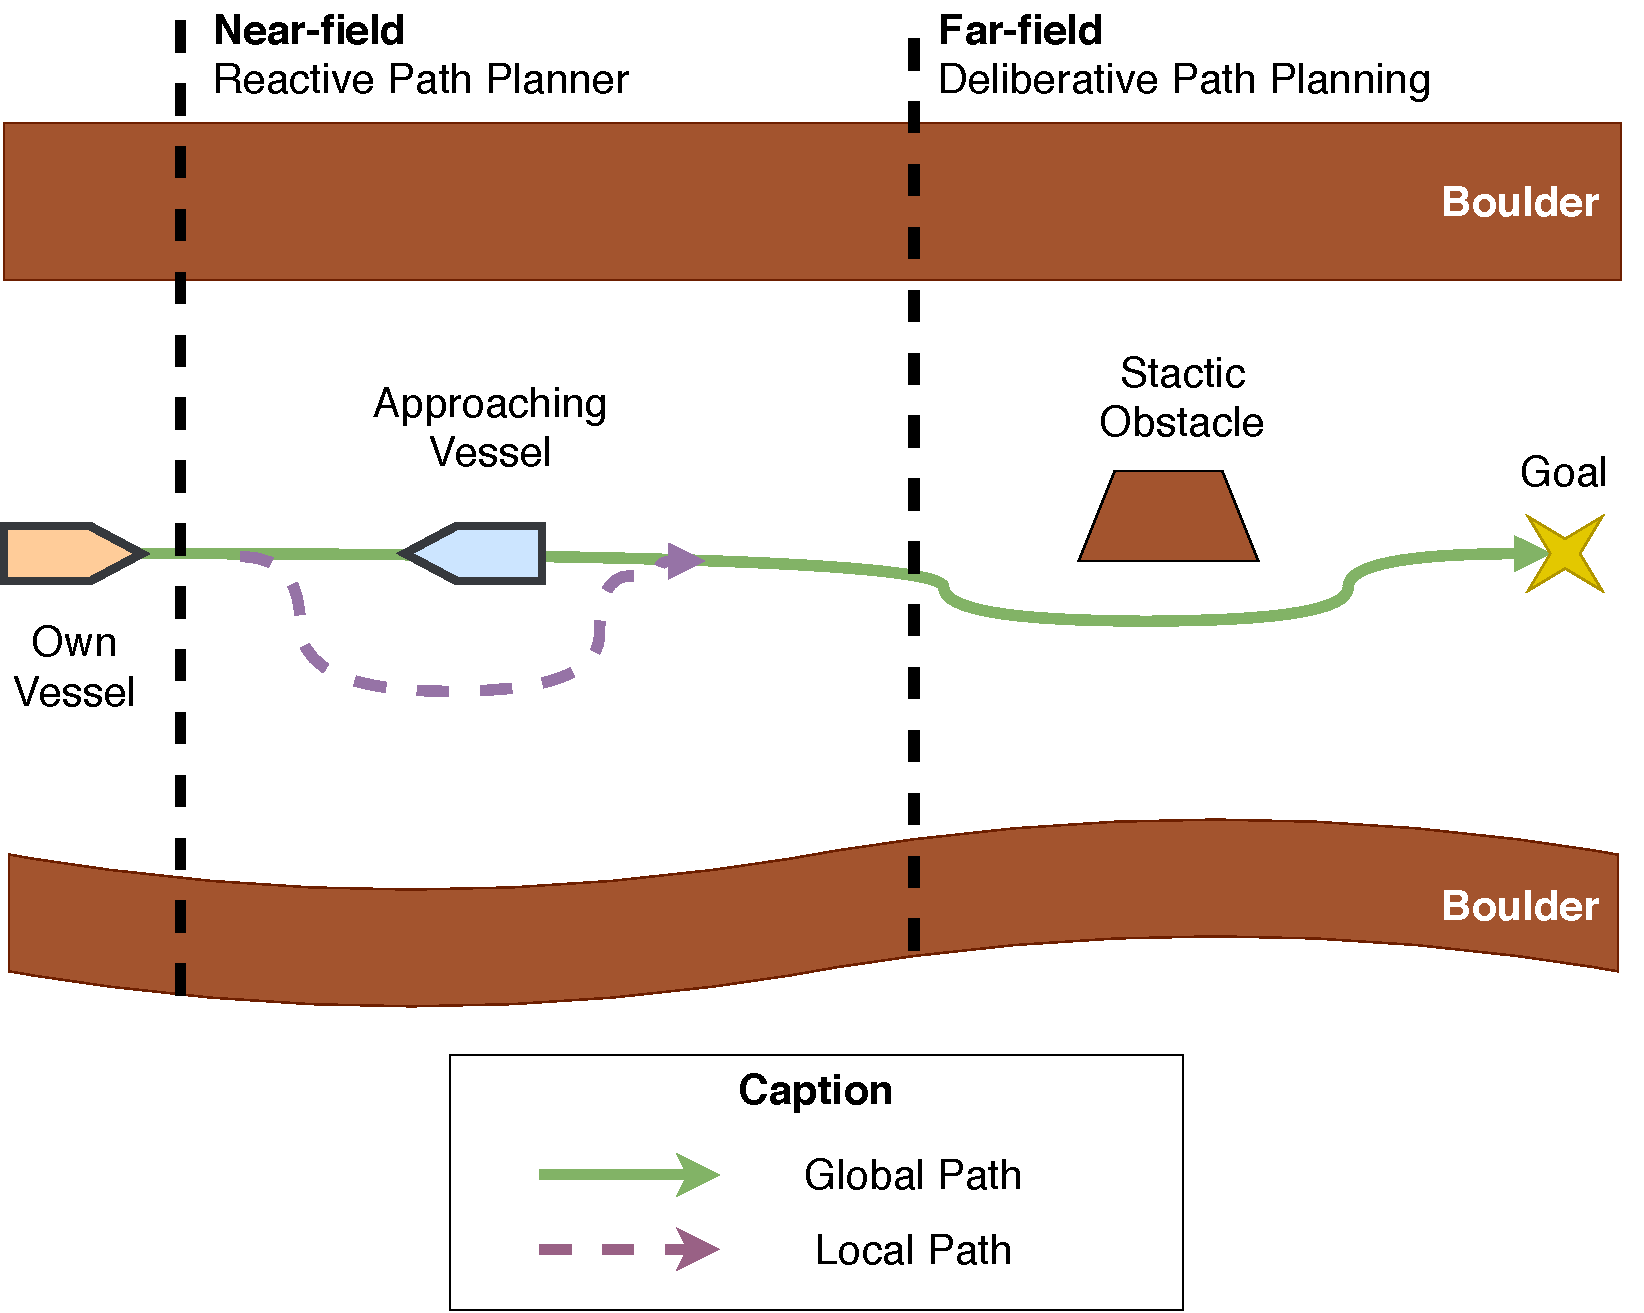
\includegraphics[scale=0.6]{figs/Chap2/GlobalLocalPath.pdf}
        \caption{Global and local paths.}
        \label{fig:chap2_globallocalpath}
    \end{figure}

    %%%%%%%%%%%%%%%%%%
    % Grammarly: 100/100
    %%%%%%%%%%%%%%%%%%
    In general, static information about the environment, such as islands, and coasts, are extracted from nautical charts, topography charts, and offline available maps. While dynamic information about the environment, such as unknown static obstacles and other vessels, is acquired in run-time by the navigation system. Also, the guidance system depends on a world representation (i.e., cost maps) for running its main component, the path planner.

    \subsection{Navigation System}
    
    %%%%%%%%%%%%%%%%%%
    %
    %%% Navigation   
    %
    %%% Grammarly: 99/100
    %%%%%%%%%%%%%%%%%%
    The navigation system is responsible for the determination of the current state of the \ac{USV} (e.g., position, velocity, orientation, and acceleration) and environment perception (e.g., static and dynamic obstacles, other vessels, wind speed, and water current). For \ac{USV}'s state estimation, the navigation system can use GPS, \ac{IMU}\footnote{For more information read https://en.wikipedia.org/wiki/Inertial\_measurement\_unit}, and compasses. Regarding environment perception, static information about the environment is extracted from nautical charts and topographic maps. While, dynamic information about the environment is acquired in real-time sensing by the navigation system through the usage of cameras, \ac{LIDAR}\footnote{For more information read https://en.wikipedia.org/wiki/Lidar}, radar, and \ac{AIS}. \ac{AIS} allows automated message exchange between vessels, facilitating the identification of location, velocity, course, path, dimension, and type of \acp{AV}.
    
    \subsection{Control System}
    %%%%%%%%%%%%%%%%%%
    %
    %%% Control
    %
    %%% Grammarly: 100/100
    %%%%%%%%%%%%%%%%%%
    The control system is responsible for the generation of actuation commands that change the \ac{USV}'s state. For an airboat (as shown in Figure \ref{fig:chap2_airboat}), for example, the control system will generate commands to change the rotation and gain of the fan. While for a differential boat (as shown in Figure \ref{fig:chap2_diffboat}), the control system will generate a gain command for each thruster. The control system determines actuation commands, considering the trajectory generated by the guidance system.
    
    \begin{figure}[H]
    \centering
    
        \begin{subfigure}[b]{0.44\textwidth}
            \centering
            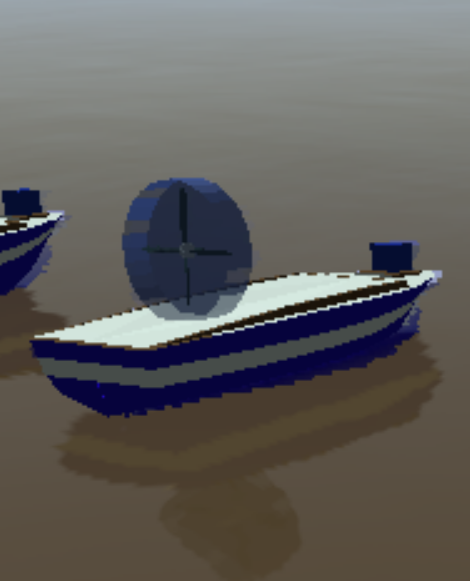
\includegraphics[scale=0.44]{figs/Chap2/airboat.png}
            \caption{Airboat with fan}
            \label{fig:chap2_airboat}
        \end{subfigure}
        \hfill
        \begin{subfigure}[b]{0.52\textwidth}
            \centering
            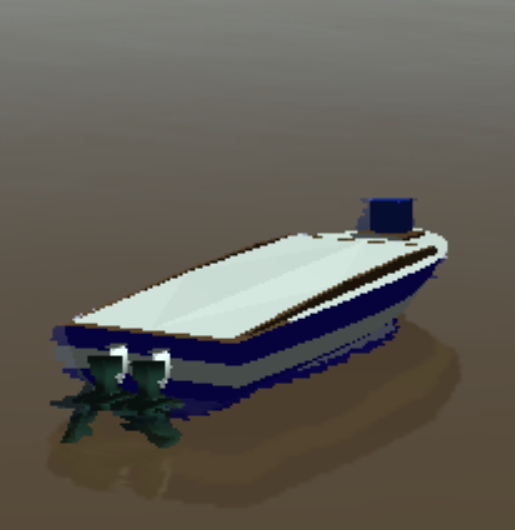
\includegraphics[scale=0.48]{figs/Chap2/diffboat2.png}
            \caption{Differential boat with two thruster}
            \label{fig:chap2_diffboat}
        \end{subfigure}
    
    \caption{Example of vessels and different propellers. Both vessels are simulated versions of Platypus~\cite{PlatypusLLC} boats we have in our laboratory.}
    \label{fig:boats}
    \end{figure}

\section{COLREGS}
\label{sec:colregs}

    %Campbell2012Rule
    % Human error, both active and latent, are said to cause marine collisions in an estimated 89-96\% of cases (Roth-blum (2000)), for instance the catastrophic MVDo˜na Paz ferry collision with the MTVector. An intelligent Obstacle Detection and Avoidance (ODA) system can potentially eliminate the issues caused by poor judgement or failure to react promptly.

    %%%%%%%%%%%%%%%%%%
    %%% Grammarly: ??/100
    %%%%%%%%%%%%%%%%%%
    \ac{COLREGS}\cite{COLREGS} stands for "International Regulation for Preventing Collisions at Sea, 1972", sometimes cited as "COLlision REGulations at Sea" or "Convention on the International Regulations for Preventing Collisions at Sea" - in this work we adopted the latter. The definitions declared on the \ac{COLREGS} are controlled, updated, and of responsibility of the \ac{IMO}. Briefly, the \ac{COLREGS} defines the rules that must be followed by vessels upon waters to avoid collisions when encountering another vessel. 
    The \ac{COLREGS} are adopted by the United Nations as a global convention and must be respected by every country.
    
    % Some rules are related to possible or mandatory features required for a \ac{USV} system, such as 9, 10, 13, 14, 15, 16, 17, and 18. Also, other rules are related to structural requirements for \ac{USV}s in real-world trials, such as 23, and 33.
    %AMA tu sabe q o leitor vai ficar boiando totalmente aqui pois ele nao faz ideia o que sao as regras 23 e 33, por exemplo.
    %DJ: removed
    
    %%%%%%%%%%%%%%%%%%
    %%% Grammarly: 99/100
    %%%%%%%%%%%%%%%%%%
    \ac{COLREGS} rules were not defined considering autonomous systems such as \ac{USV}s. They were written to be interpreted by well-experienced sailors and imply the usage of their experience and common sense. There are gaps to be filled and subjective or ambiguous definitions to be addressed, making the development of a \ac{COLREGS}-compliant \ac{USV} guidance system challenging.
    %%%%%%%%%%%%%%%%%%
    %%% Grammarly: 100/100
    %%%%%%%%%%%%%%%%%%
    Below we describe the four main encounters presented in \ac{COLREGS} (illustrated in Figure \ref{fig:chap2_encounters}), head-on, crossing from the right, crossing from the left, and overtaking.
    
    \begin{itemize}
        \item Head-On: In this situation both vessels should avoid collision going to their starboard side.
        \item Crossing from the right and crossing from the left: In this scenario, the \ac{COLREGS} defines different responsibilities for each vessel. The vessel that has the other vessel in its starboard side must give way and is responsible for collision avoidance. The vessel that has the other vessel in its port side must keep its course without significant changes. In a critical situation, where the give-way vessel seems not able to avoid the collision, the keep vessel should act to avoid.
        \item Overtake: In this scenario the vessel overtaking another, can freely decide which side to go and must avoid generating another crossing situation.
    \end{itemize}
    
    \begin{figure}[H]
        \centering
        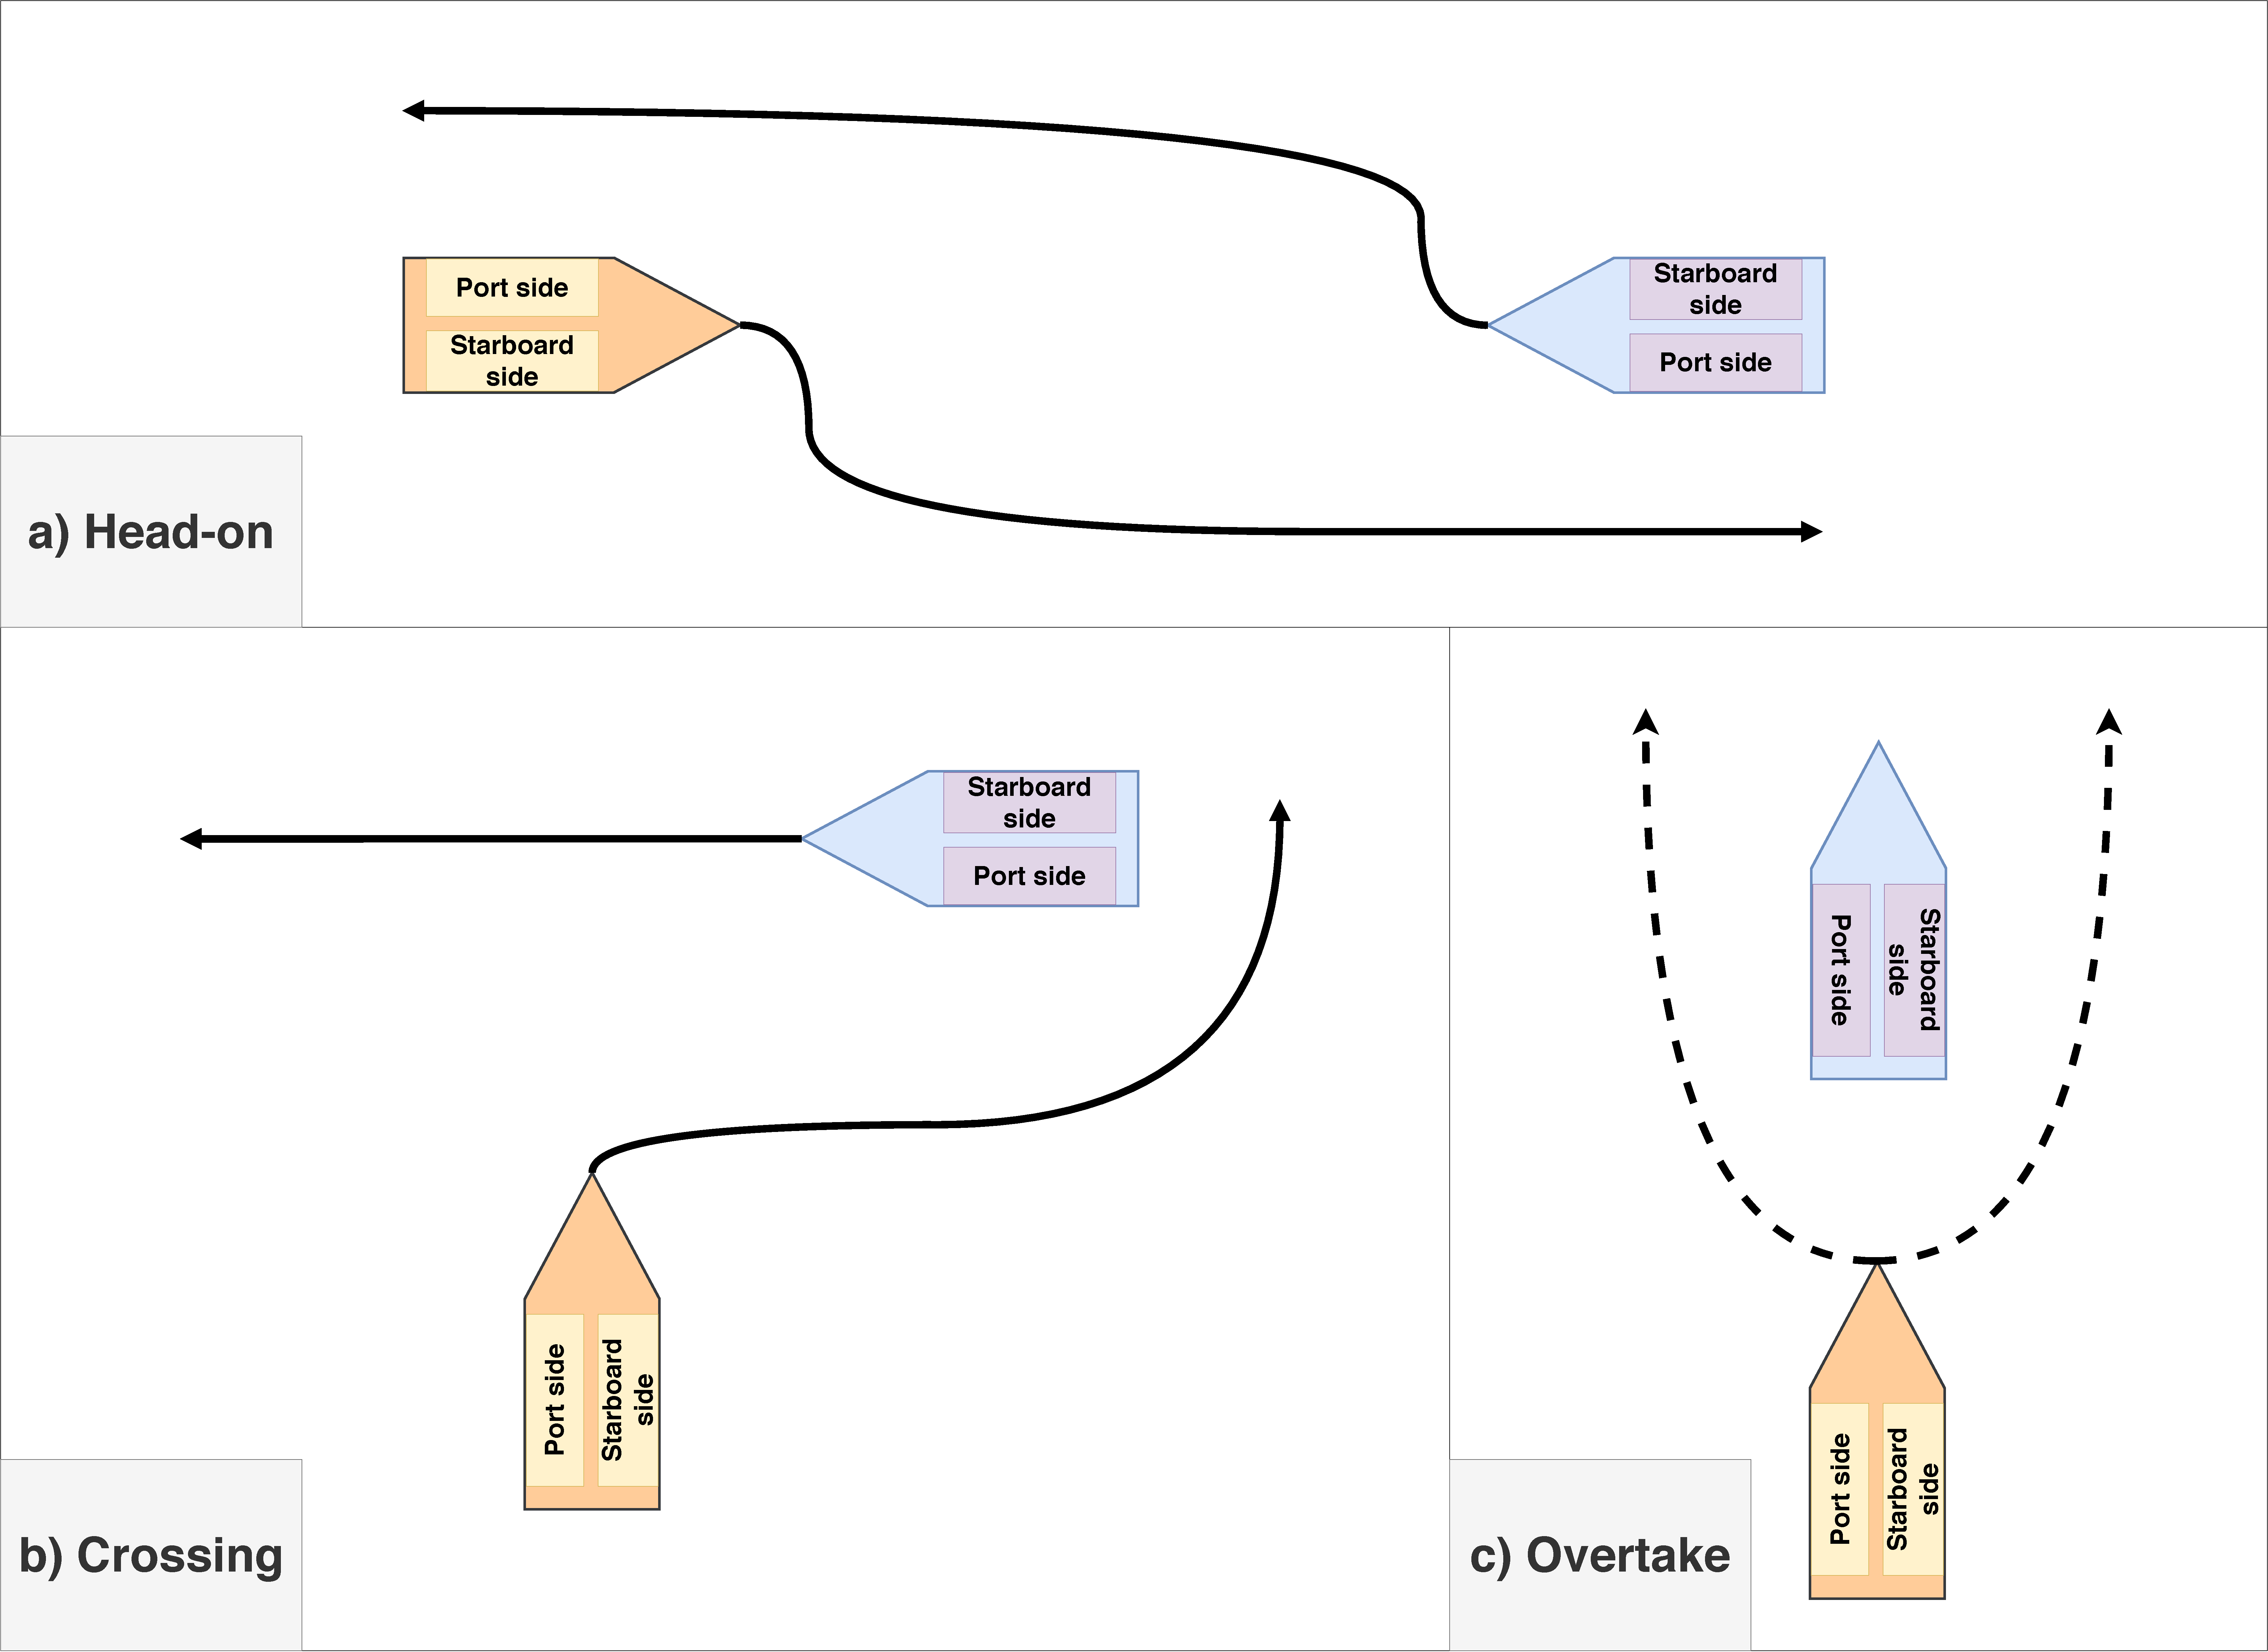
\includegraphics[scale=0.125]{figs/Chap2/Encounters.pdf}
        \caption{Possible encounters between two vessels discussed in the \ac{COLREGS}. Arrows indicate the behavior that must be performed by the vessels. In c) there is two possible paths for the orange vessel. }
        \label{fig:chap2_encounters}
    \end{figure}

    % \section{ROS}
    % \section{A*}
    
% \section{A*}

% A-star method, or simply A*, is a basic path planning algorithm in various fields, which uses heuristics to find the optimal path. A* algorithm is correct, complete and optimal. The meaning of correctness is that there are no obstacles on the computational path. Completeness means that a path can be found , if feasible path exists. Optimally means that it is able to calculate the shortest path from the start point to the goal point.
% Define an evaluation function for the A*
% f (n) = g(n) + h(n) (1)
% where
%  g(n) is the cost of the path from the start point to node
% n found so far. g(n) is given by
% g(n) = g(n - 1) + c(n, n - 1) (2)
% where c(n,n-1) is the cost from node n-1 to its neighbor node n that calculated by using the Euclidean distance.
%  h(n) is the straight-line distance from the node n to the goal point. For predefined goal piont, the value of h(n) is constant which can be calculated in advance.
%  f(n) is an estimate of the cost of an optimal path from start point via node n to the goal point.
% There are two important priority queues in the A* algorithm, open list and close list. Open is a stable priority queue, which storages nodes with the key f value in ascending order. Close storages expanded nodes to ensure that each node is only expended once. The lowest f value in the Open will be selected as he current node, and the path is found when the current node is goal point. \cite{Wang2018Hybrid}

% \section{Proportional Controller}
% \section{Euclidian Distance}
% \section{Steering Angle}
% \section{Atan2}
    
% VO because the algorithms collect all the velocities that result in collisions and present a set of collision-free velocities for human/machine, which facilitates human/machine to search for the best option.

% The advantages of the VO algorithms have been noticed by researchers in maritime engineering. The idea of VO algorithms had ap- peared in the 1980s, named as Collision Threat Parameter Area (CTPA) (Degre and Lefevre, 1981; Lenart, 1983). Subsequently, Pedersen et al. (2003) showed that this method can provide a better support for the Officer On Watch (OOW) in collision prevention comparing with tra- ditional Automatic Radar Plotting Aid (ARPA). Later on, a series of studies proposed to use VO/CTPA algorithms for collision avoidance in various scenarios, e.g. restricted waters (Szlapczynski and Szlapczynska, 2017), multiple-ship (Szlapczynski, 2008), incorporating with regulations (Zhao et al., 2016), and unmanned ship (Kuwata et al., 2014). In (Huang et al., 2018), the algorithms which presume the target-ship keeps constant velocity, are concluded as a special case of the VO algorithm, called linear VO (LVO) algorithm. Details about the existing applications of VO algorithms in the maritime domain are addressed in Section 2.3.

  % \subsubsection{Behavior-based systems}
        
        %% Benjamin2004COLREGS
        % The origin of behavior-based systems is commonly attributed to Brooks' "subsumption architecture" in [R. Brooks, “A Robust Layered Control System for a Mobile Robot”, IEEE Journal of Robofics and Automation, RA-2(1):14-23, April 1986]. Since then, it has been used in a large variety of applications including: indoor robots, e.g., [l, 2, 7, 9, 13, 14, 17, 19, 201, land vehicles, e.g., [16], planetary rovers, e.g., [12, 181, and marine vehicles, e.g., [3,4,6,8, 15] 
        
        %% Benjamin2004COLREGS
        % Action selection, as indicated in Fig. 1, is the process of choosing a single action for execution, given the outputs of the behaviors. The "action space" is the set of all possible distinct actions, e.g., all speed, heading and depth combinations for a marine vehicle.
        
        %% Benjamin2004COLREGS
        % Its influence depends on whether the rule associated with the behavior applies to the current situation. The output of each behavior is an objective function that rates all possible actions with respect to the corresponding COLREGS rule. The detaiIs of solving multi-objective optimization problems in the interval programming model can be found in [3]
        
    % \subsubsection{Genetic Programming}
    % Genetic Programming is an automated programming technique, based on the automated composition of 
    % a set of functional programming blocks into an increasing amount of modules for 
    % generation of a structured solution with the desired functionality. 
    % Genetic Programming explore a random combination of functional blocks through the generation of expressions 
    % tree where each node is represents a functional block. Solutions are generated by combination, mutation and
    % crossover between subtrees.
    
    % \subsubsection{A*}
    
    % The A* algorithm is a classical grid-based methodology which has been widely applied in different shapes and forms. It uses s heuristic method to focus the search towards the goal position. Using an edge cost and a heuristic based on the Euclidean distance, the A* algorithm can find the shortest paths \cite{Hart1972Formal}. For the classical A* algorithm, its scalability is limited by its memory requirements. It stores all explored nodes of a search graph in the memory, using an Open List to store nodes on the search frontier and a Closed List to store already-expanded nodes.
    
    % Depending on the size of the grid map, a large number of nodes may have to be searched at any given time. Thus, repeatedly searching through these lists can slow down the application significantly. Hence, it is not suitable for real-time engineering applications requiring on-the-fly computations.
    
    % Search space
    
    % \subsubsection{Occupancy Grid}
    % \subsubsection{Velocity Obstacle} \unsure[inline]{maybe remove from here and explain only in the literature review}
    
    % The velocity obstacle (VO) approach has been adopted by several researchers for moving hazard avoidance. Since it was first proposed in 1998 for robot motion planning [10], several extensions to VO have been made.  VO approaches generate a cone-shaped obstacle in the velocity space (hence the name velocity obstacles) and ensure that there will be no future collisions as long as the robot’s velocity vector is outside the VO. To identify the risk of future collisions, one could predict both the pose of the moving hazard and the pose of the robot for several time steps into the future, and perform collision checks using their configurations at each time slice. This approach has the advantage that it can check collisions of vehicles following arbitrary trajectories. However, because it needs to perform collision checks at many time slices, the computational load becomes very high.

    % On the other hand, VO makes a first-order (i.e., linear) prediction, and the collision check is done in the velocity space. Since a single collision check accounts for collision checks at all future times (due to the linear velocity assumption), VO is very fast to compute and extends well to high-speed operations with short reaction time. Furthermore, its simplicity is suited for our behavior-based control architecture.
    
    % \subsubsection{Line of Sight}
    % \subsubsection{Direction Priority Sequential Selection} \unsure[inline]{maybe remove from here and explain only in the literature review}
    % \subsubsection{Rule-Rapairing A*} \unsure[inline]{maybe remove from here and explain only in the literature review}
    % \subsubsection{Virtual Force Field}
    % \subsubsection{Fuzzy Logic}
    % \subsubsection{Interval Programming}
    % \subsubsection{Closest Point of Approach}
        % One is using various indicators to measure a collision risk and find associated evasive actions that keep the risk at an acceptable level. Two widely used indicators, Distance to CPA (DCPA) and Time to CPA (TCPA), are based on the concept of closest point of approach (CPA) (Kearon, 1979).
    % \subsubsection{Occupancy Grid}